\chapter{Design patterns}

\setcounter{section}{3}
\setcounter{subsection}{0}

\subsection{Modularity}

Frameworks such as Sproutcore and Angular.js allow applications to be divided into smaller components \cite{sproutcore_getting_started} \cite{angularjs_modules}. In bigger projects is modularity a key aspect to improve maintainability. If one component cannot be replaced without affecting the other components the application will easily become hard to manage in the long run. When each component solves a specific task they can also be developed in parallel, it also becomes easier to test and maintain the entire application \cite{addy_osmani_modular_js}. A modular pattern is well suited since a website is naturally divided into several different pages where each page has its own functionality.

Another feature of a modular design is that it allows for code re-usage. If a module written in one project could be used in a new project without any major changes the efficiency would be improved. It also becomes easier to achieve high-quality code since already tested code can now be re-used.

\subsubsection{The module pattern}
By using a modular design pattern the architecture can be formed in a way that allows smaller components to be grouped together into a common module. The idea behind the module pattern is to provide private and public encapsulations, like normal classes. There are several ways of implementing this pattern in Javascript. However, important to note is that all these implementations only emulates traditional classes since Javascript doesn't support classes and access modifiers \cite[p. 27]{addy_osmani_design_patterns}. Private members can however easily be emulated by hiding them in a function scope that only is available within the instance. An example of a module implementation in Javascript is described in listing \ref{code_module_example}.

\lstset{frame=single, caption=A simple example of how to implement a module in Javascript using the function literal notation., label=code_module_example, captionpos=b, tabsize=2}
\begin{framed}
\begin{lstlisting}
function MyModule() {
	// Private variables
	var private_variable = 0;

	// Private methods
	var private_method = function() {
		return private_variable;
	};

	// Public variable
	this.public_variable = 10;

	// Public methods
	this.public_method = function() {
		return private_variable;
	};
}
\end{lstlisting}
\end{framed}

\subsubsection{The singleton pattern}
The singleton pattern restricts the number of instances of a class to one single instance. This is suitable for when writing components that are supposed to have a unique instance which is used across the entire system. This tends to be common in web applications, typical examples are API, messaging and debug components. Along with this the singleton pattern has the same advantages as the traditional module pattern.

\subsubsection{Inheritance}
Class inheritance is an important aspect of a modular pattern. In Javascript a prototype-based inheritance model is used \cite[p. 199]{js_def_guide}. An example of how the prototype-based inheritance model works in Javascript is shown in listing \ref{code_inheritance}.

\lstset{frame=single, caption=Prototype-based inheritance in Javascript. Child inherits from Parent., label=code_inheritance, captionpos=b, tabsize=2}
\begin{framed}
\begin{lstlisting}
// Inheritance implementation
function extend(Child, Parent) {
	// Let Child inherit from Parent
	Child.prototype = new Parent();
	Child.prototype.constructor = Child;
}

function Parent() {
	this.method1 = function() {
		return "Method 1 - Parent";
	}
	this.method2 = function() {
		return "Method 2 - Parent";
	}
}
function Child() {
	this.method1 = function() {
		return "Method 1 - Child";
	}
}
extend(Child, Parent);

var pi = new Parent();
pi.method1(); // "Method 1 - Parent"
pi.method2(); // "Method 2 - Parent"

var ci = new Child();
ci.method1(); // "Method 1 - Child"
ci.method2(); // "Method 2 - Parent"
\end{lstlisting}
\end{framed}

\subsubsection{Decorating modules}

There is sometimes a need for instantiating the same module with different amount of properties. When the number of properties grows subclassing will often become impractical since a new class for each combination of options needs to be created. The decorating pattern aims to solve this problem. It is commonly used by Javascript developers since it can be implemented transparently \cite[p. 70]{addy_osmani_design_patterns}. The real value of using this pattern is the code re-usage. By letting a module be instantiated with options it will make it generic and can easily to be shared between projects.

% TBD: \hl{More desc maybe needed?}

\subsection{Communication between modules}
To provide a modular system some kind of interface is needed. In other languages like Java the purpose of interfaces is to describe what methods must be implemented so that other modules know what to expect. The advantage of using well defined interfaces is that a module becomes easy to use, self-documented and promotes code re-usability \cite[p. 65]{addy_osmani_design_patterns}. The drawback is that Javascript doesn't come with any built in support for native interfaces, and since it is a loosely typed language some kind of validation is needed \cite[p. 65]{addy_osmani_design_patterns}. The validation is simply needed in order to make sure that the correct type of data is sent to the module. Since this is done during runtime this will affect the performance of the system, in a compiled language this would not be a problem since it would be done during compilation.

Instead of directly calling a method on a class instance through an interface the observer pattern can be used. It allows a module to register on events from other modules. When something interesting happens the responsible module can inform its subscribers about it. This allows for a more flexible interface design and will make the modules more independent of each other \cite[p. 38]{addy_osmani_design_patterns}. If one module fails to deliver a message the entire system will not crash, only the specific functionality that depended on that message will be affected.

Another possibility to get more loosely coupled modules is to use the command pattern as communication between the modules. Instead of calling methods directly on an instance every class will inherit a generic execution-function. This function will take a string as argument of what method to run. This protects the system from crashing if a method is called that is not implemented. For compiled languages this is not a relevant issue, but for interpreted languages such as Javascript there is no compiler that can help. An example how the command pattern can be implemented and used can be seen in listing \ref{code_command_example}.

\lstset{frame=single, caption=An example of how the command pattern can be implemented and used in Javascript., label=code_command_example, captionpos=b, tabsize=2}
\begin{framed}
\begin{lstlisting}
// The CommandPattern prototype
function CommandPattern() {
	this.execute = function(method) {
		if(typeof(this[method]) === 'function') {
			return this[method].apply(this,
				[].slice.call(arguments, 1));
		}
		return false;
	}
};

// An example module
function MyModule() {
	this.myMethod = function(arg1, arg2) {
		console.log(arg1 + " " + arg2);
	};
};

// Let MyModule inherit from CommandPattern
MyModule.prototype = new CommandPattern();
MyModule.prototype.constructor = MyModule;

// Create an instance of MyModule
var instance = new MyModule();

// Run myMethod() on instance with foo and bar as arguments
instance.execute("myMethod", "foo", "bar");
\end{lstlisting}
\end{framed}

\subsection{MVC - Model-View-Controller}

MVC, Model-View-Controller, originated from the early days of Smalltalk-80 \cite[p. 4]{elem_reuse_oo}. The pattern is commonly used when creating user interfaces. The main idea behind MVC is to separate the presentation layer from the data layer. It's basically a pattern that can be constructed by combining the composite-, observer- and strategy-pattern all together \cite{head_first}. MVC divides the design into models, view and controllers \cite[p. 14]{elem_reuse_oo}:

\begin{itemize}
	\item Model - A record of data, completely ignores the UI
	\item View - Presents the model in a graphical form
	\item Controller - Takes user input and figures out what to do with it
\end{itemize}

The view observes the model for changes. If the model changes the view is re-rendered to keep the presentation up-to-date. On user input the controller will take a decision of what to do, if this involves changing a model it will tell the model to do so. The view will then be informed about this due to its observations. This means that the controller never really care what views are rendered. The view itself is composed by several UI-elements and implements therefore the composition-pattern. Figure \ref{fig:mvc} describes the communication between the different components of the MVC pattern.

\begin{figure}[h!]
	\centerline{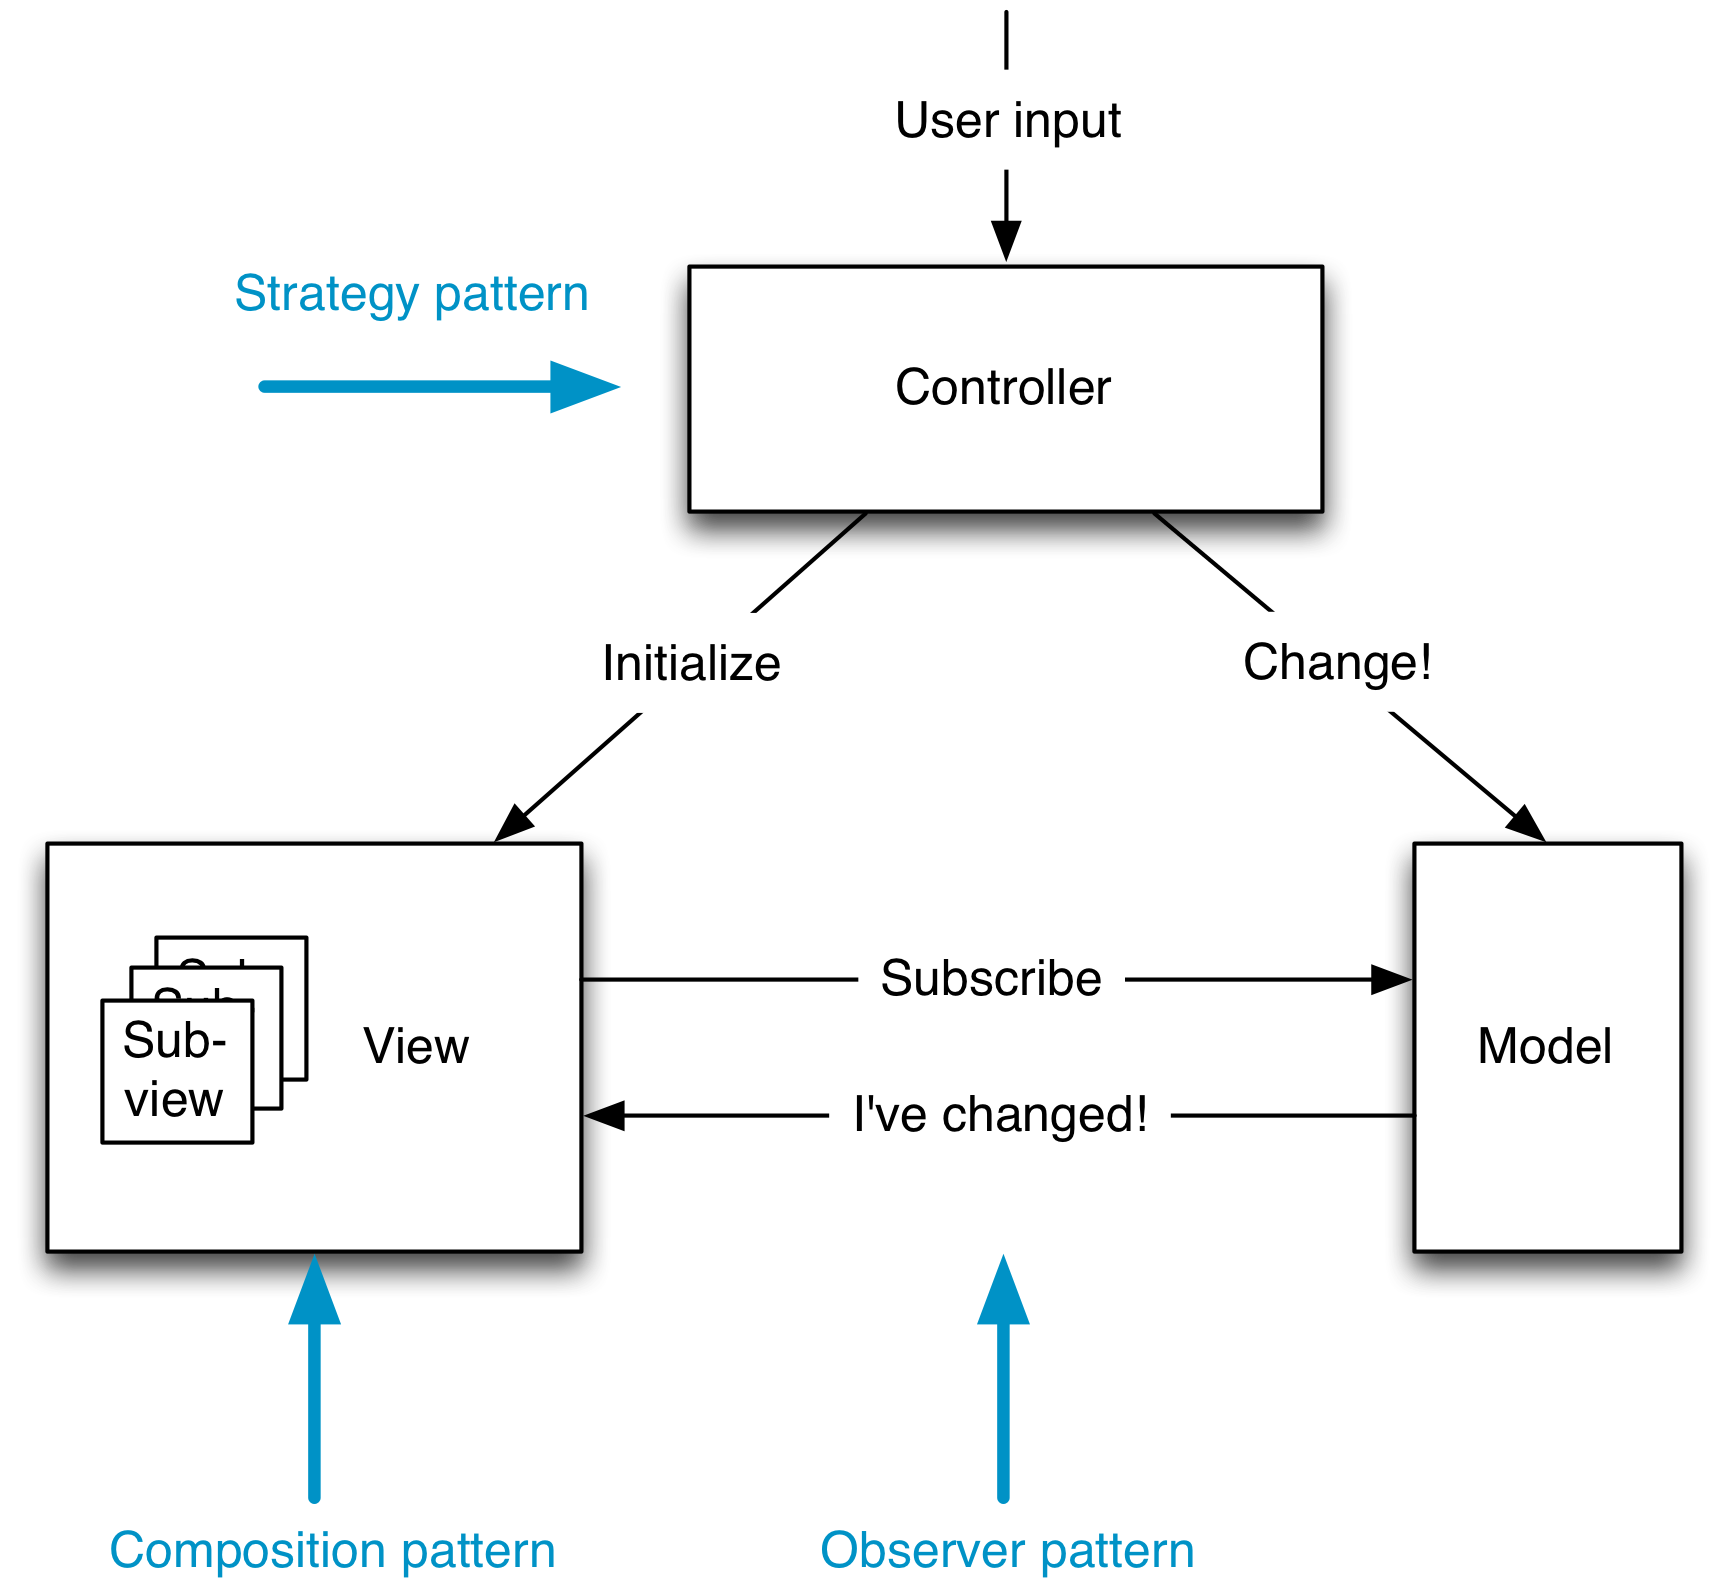
\includegraphics[width=90mm]{gfx/mvc.png}}
	\caption{Communication between the different parts of the MVC pattern.}
	\label{fig:mvc}
\end{figure}

Since MVC was designed with user interfaces in mind it also becomes a suitable choice when designing an architecture for a Javascript frontend. Most of todays Javascript-frameworks are based on MVC. Some of them are classical MVC-frameworks while others have made a few modifications.

However, MVC has a few drawbacks as well. The view often has to keep track of several different UI-specific properties. The rest of the system is not interested in these UI properties, but the view cannot operate correctly without them. An example is if an image slideshow should change image periodically, the view needs to know which the current image is so that the next one can be loaded. However, this information is useless for the rest of the system, it is only needed by the view. A combination of the model and UI properties forms a state of what is currently presented to the user. Suddenly the view is supposed to take care of both presentation logic and UI elements. They can easily become quite complex and hard to maintain. 

Also worth mentioning is MVP, Model-View-Presenter, which is a lot like the traditional MVC pattern. The main difference is that in MVP the user actions are captured by the view that raises an event, compared to MVC where the controller captures the user actions directly. By letting the view capture the user actions the coupling between the controller and the UI-elements will be reduced, improving the ability to re-use the code.

\subsection{MVVM - Model-View-ViewModel}

MVVM is a quite new compound of design patterns, originated from Microsoft as late as in 2005 \cite{mvvm_history}. It is currently used in Silverlight as well as in a number of Javascript frameworks such as KnockoutJS, Kendo MVVM and Knockback.js \cite{mvvm_used}. MVVM is designed to make two-way data-bindings easier to implement and use. It consists of three type of components: models, views and view-models. The views and models in MVVM have the same purpose as in the traditional MVC pattern. However, the view-model binds elements in the view to a specific model. Due to the two-way data binding the controller is no longer needed since changes in the view directly correspond to changes in the model and vice-versa. Other responsibilities that the controller had in MVC moved to the view-model, such as replacing views and deciding when to fetch data from the backend.

The main drawback of MVVM is that the view-model quickly grows and becomes complex to maintain since it has quite a lot of responsibilities \cite{mvvm_drawbacks}. Another drawback of the MVVM pattern is that it is designed to be used together with two-way data-bindings which easily can make it overkill for smaller systems with a relative few number of UI elements. Other patterns, like MVC or MVP, might in that case be a better alternative.
